\section*{Atypical rDNA operon structure}

Ribosomal RNA coding regions are commonly arranged into operons consisting of a 16S rRNA, 23S rRNA, and one or more 5S rRNAs, often with various tRNAs interspersed. In the course of this study, we observed some taxa lacking this typical 16S--23S--5S rRNA operon. When rDNAs are not structured into operons, assemblies from short reads do not suffer from the issue of long repeats. We developed a module called \texttt{structure} for plotting rDNAs across a collection of genomes; this is available for riboSeed as of version 0.4.50.  Figure \ref{fig:atypical} show the operon arrangement of a few examples of organisms exhibiting atypical operon structure. For comparison, the rDNAs in the reference strains used in this study are shown in Figure \ref{fig:typical}.  Work to characterize this anomaly is underway in our lab.

\begin{figure}[H]
  \centering
  \hspace*{0cm}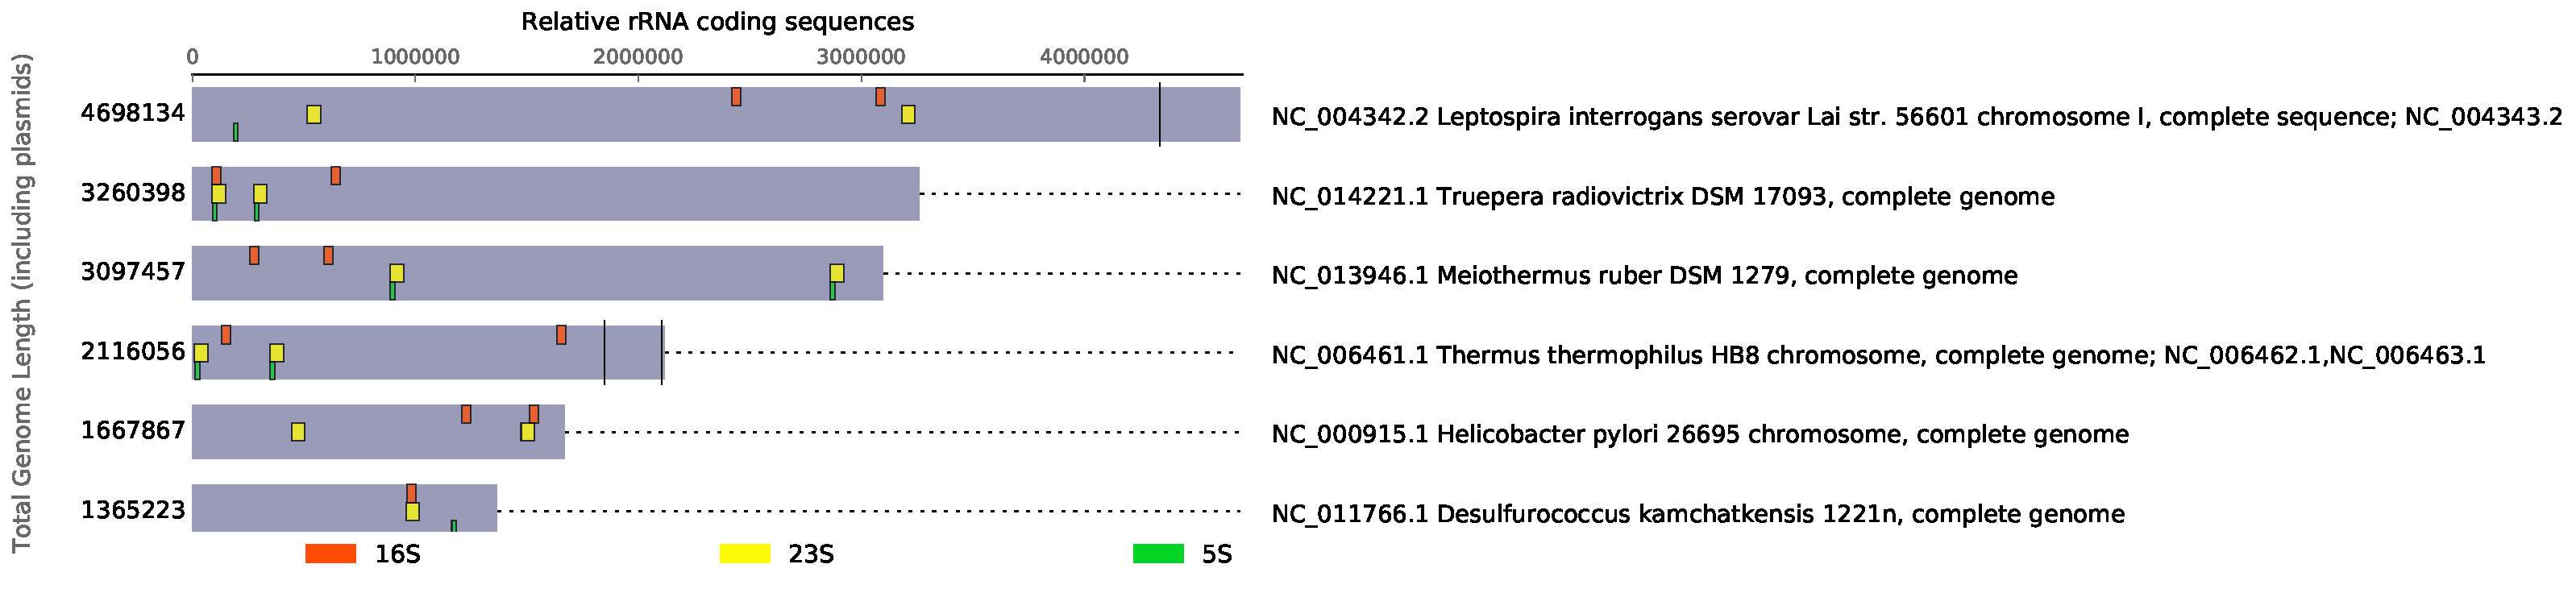
\includegraphics[width=1.0\textwidth]{odd_rDNA_relative_locations}
  \caption{Atypical rDNA operon structure in select taxa. rRNA lengths are not shown to scale. Note that the NCBI record for \textit{Helicobacter pylori} (NC\_000915.1) shows a 5S rRNA not detected by Barrnap. }
  \label{fig:atypical}
\end{figure}

\begin{figure}[H]
  \centering
  \hspace*{0cm}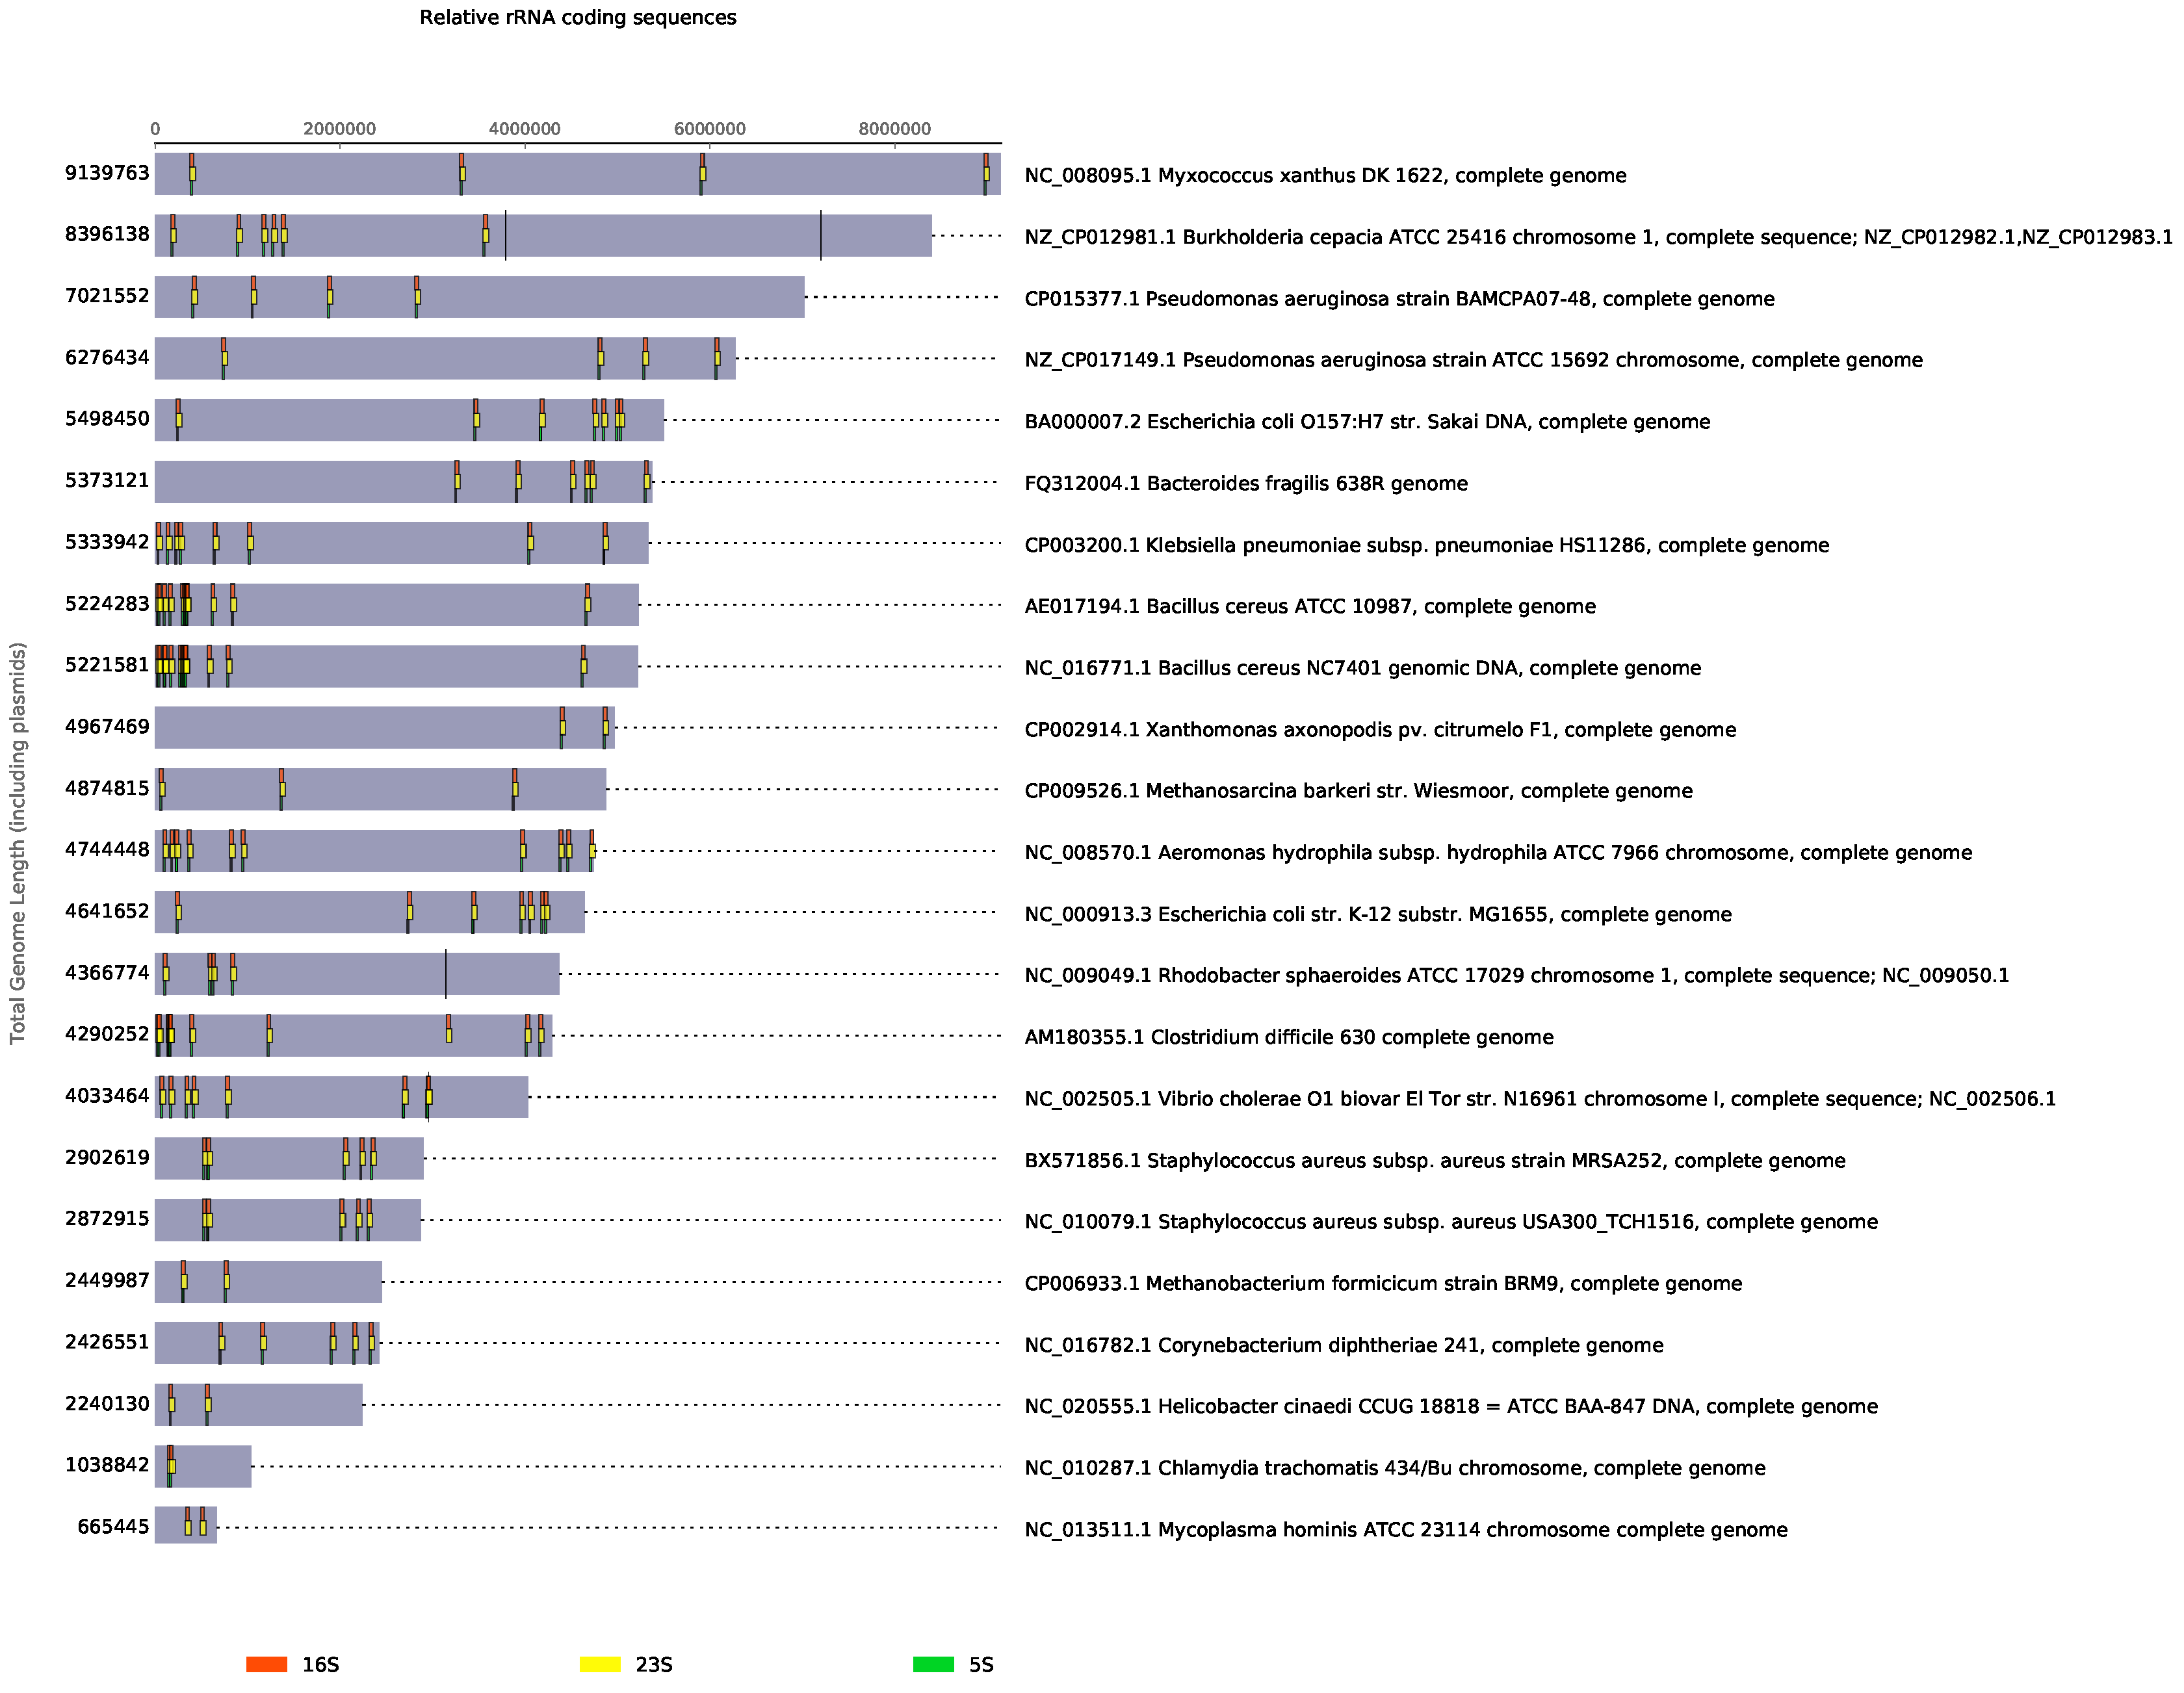
\includegraphics[width=1.0\textwidth]{normal_rDNA_relative_locations}
  \caption{Typical rDNA structure for strains used in this study.}
  \label{fig:typical}
\end{figure}
